\begin{figure}
    \centering
    \begin{subfigure}[b]{0.485\linewidth}
        \centering
        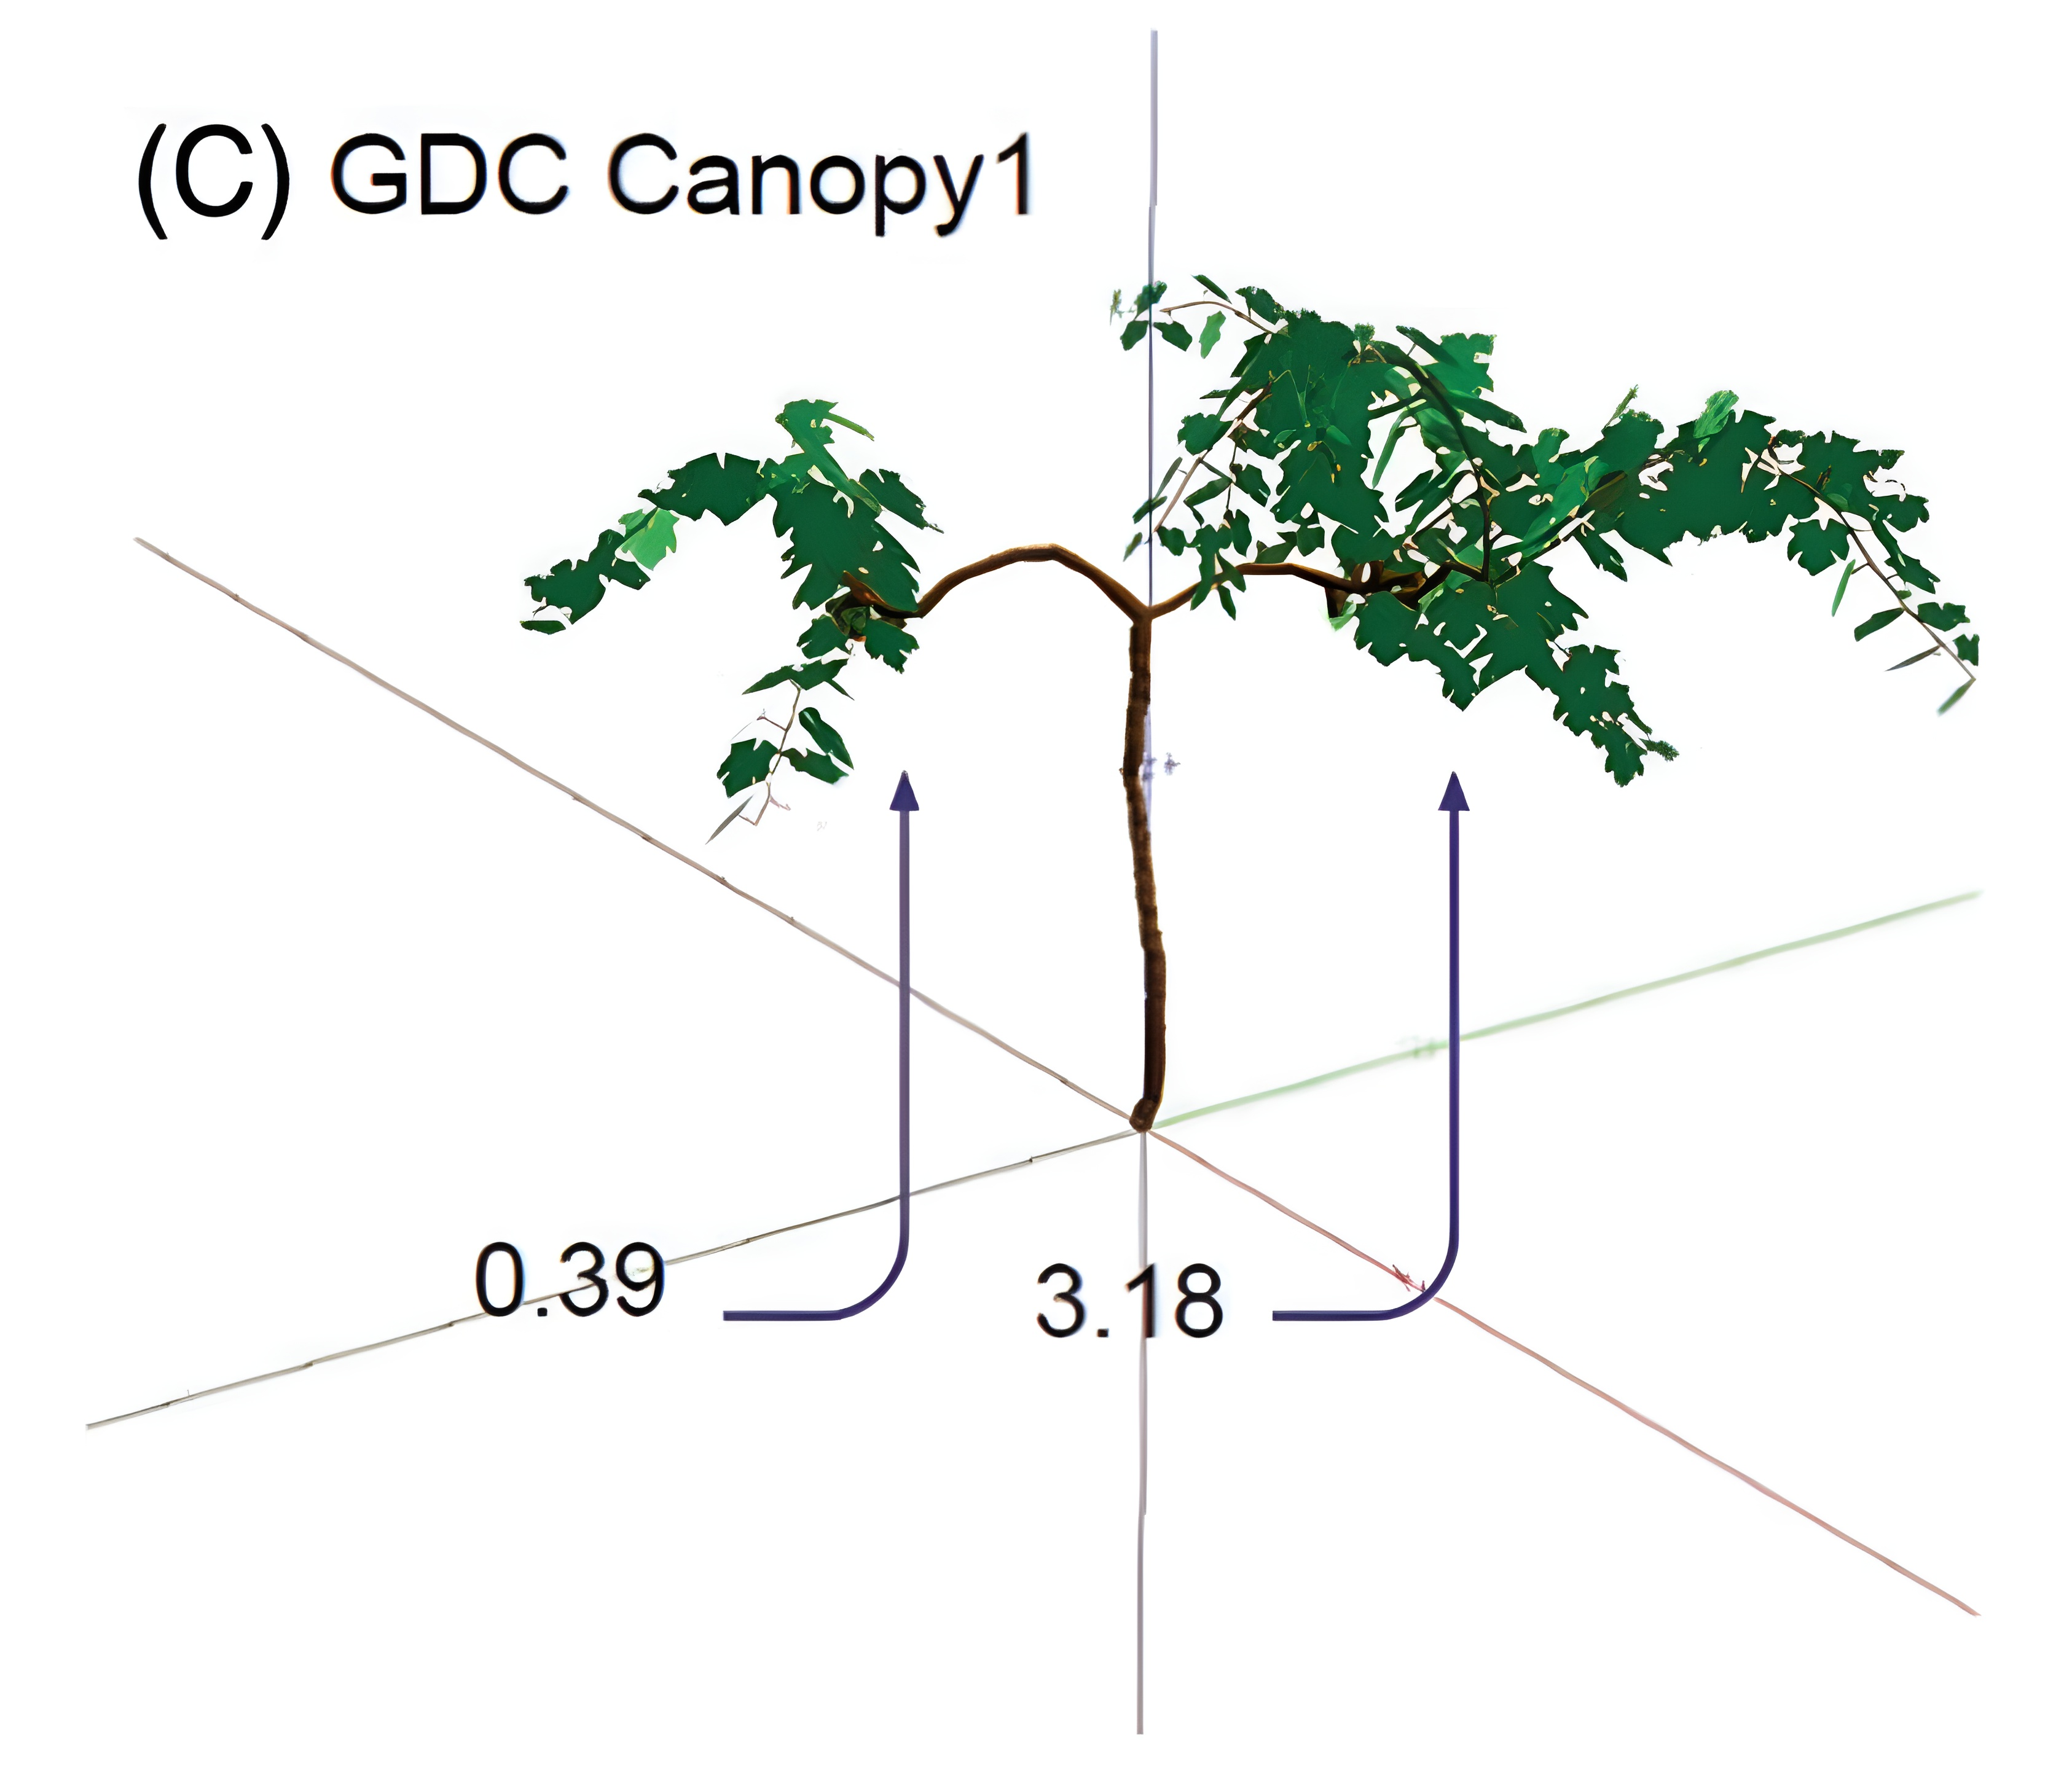
\includegraphics[width=\linewidth,height=\linewidth,keepaspectratio]{img/hydroshoot_can1_upscaled.jpg}
        \caption{HydroShoot}
        \label{fig:hydroshoot-archi}
    \end{subfigure}
    \hfill
    \begin{subfigure}[b]{0.485\linewidth}
        \centering
        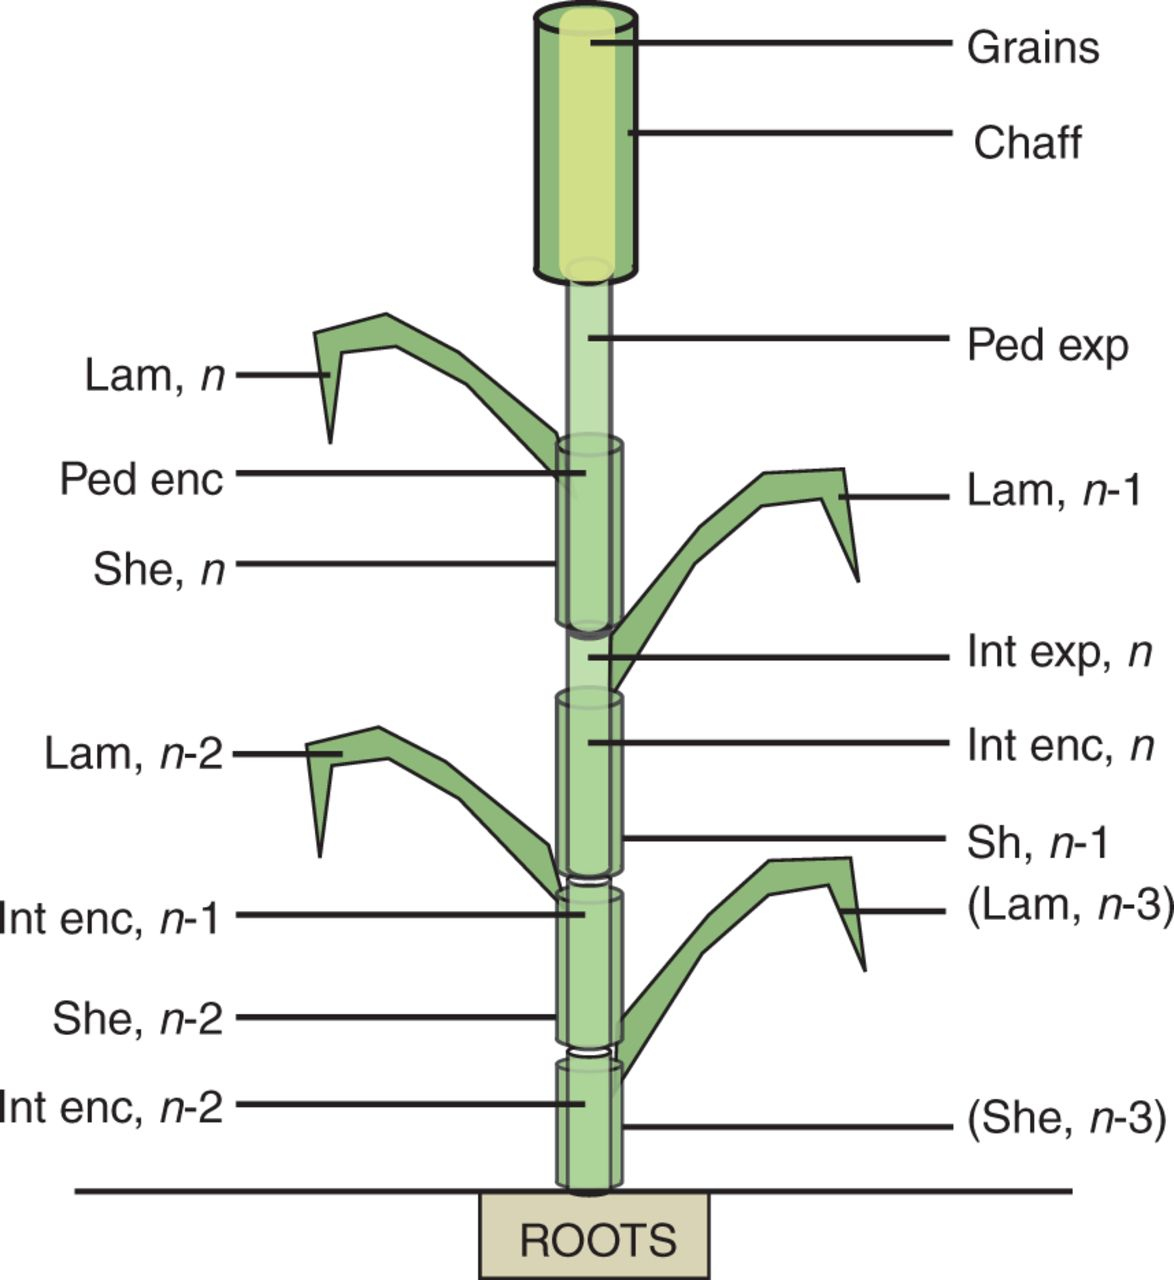
\includegraphics[width=\linewidth,height=0.85\linewidth,keepaspectratio]{img/cnwheat_architecture.jpeg}
        \caption{CN-Wheat}
        \label{fig:cnwheat-archi}
    \end{subfigure}
    \caption[FSPMs selected for use in experiments in this work.]{
            FSPMs selected for use in experiments in this work. 
            (\subref{fig:hydroshoot-archi}) A grapevine specimen from HydroShoot with the canopy trained in the ``Geneva Double Curtain'' configuration.  This figure is reused from \citet{albasha_hydroshoot_2019} under the CC BY 4.0 license.
            (\subref{fig:cnwheat-archi}) The architecture of the CN-Wheat model. This figure is reused from \citet{barillot_cn-wheat_2016} with permission from the publisher (Copyright 2016 Oxford University Press).
    }
    \label{fig:fading_memory_experiments}
\end{figure}

% CC BY 4.0 license